\documentclass[english,11pt,usenames,dvipsnames]{beamer}

\DeclareMathOperator{\Cov}{Cov}
\DeclareMathOperator{\Var}{Var}
\DeclareMathOperator{\E}{\mathbb{E}}
\DeclareMathOperator{\Proba}{\mathbb{P}}

\newcommand{\Covb}[2]{\ensuremath{\Cov\!\left[#1,#2\right]}}
\newcommand{\Eb}[1]{\ensuremath{\E\!\left[#1\right]}}
\newcommand{\Pb}[1]{\ensuremath{\Proba\!\left[#1\right]}}
\newcommand{\Varb}[1]{\ensuremath{\Var\!\left[#1\right]}}

% norm
\newcommand{\norm}[1]{\| #1 \|}

\newcommand{\indep}{\rotatebox[origin=c]{90}{$\models$}}





\usepackage{mathptmx,amsmath,amssymb,graphicx,bibentry,bbm,babel,ragged2e}

\makeatletter

\newcommand{\noun}[1]{\textsc{#1}}
\newcommand{\jitem}[1]{\item \begin{justify} #1 \end{justify} \vfill{}}
\newcommand{\sframe}[2]{\frame{\frametitle{#1} #2}}

\newenvironment{centercolumns}{\begin{columns}[c]}{\end{columns}}
%\newenvironment{jitem}{\begin{justify}\begin{itemize}}{\end{itemize}\end{justify}}

\usetheme{Warsaw}
\setbeamertemplate{footline}[text line]{}
\setbeamercolor{structure}{fg=purple!50!blue, bg=purple!50!blue}

\setbeamersize{text margin left=15pt,text margin right=15pt}

\setbeamercovered{transparent}

\setbeamertemplate{headline}{}
\setbeamertemplate{footline}[frame number]
\setbeamertemplate{navigation symbols}{}

\@ifundefined{showcaptionsetup}{}{%
 \PassOptionsToPackage{caption=false}{subfig}}
\usepackage{subfig}

\usepackage[utf8]{inputenc}
\usepackage[T1]{fontenc}


\usepackage{tikz}

\usepackage{multirow}


\usepackage{mdframed}

\usepackage[usenames,dvipsnames]{pstricks}
\usepackage{auto-pst-pdf}


\usepackage[dvipsnames]{xcolor}


\makeatother

\begin{document}


\title{De l'endogénéité des hiérarchies dans les systèmes territoriaux complexes}

\author{J.~Raimbault$^{1,2,3}$\\
\texttt{juste.raimbault@iscpif.fr}
}


\institute{$^{1}$UPS CNRS 3611 ISC-PIF\\
$^{2}$CASA, UCL\\
$^{3}$UMR CNRS 8504 G{\'e}ographie-cit{\'e}s
}


\date{JIG 2019\\\smallskip
3 avril 2019
}

\frame{\maketitle}

%\textbf{Mots-clés : }\textit{Théories de la complexité ; théorie évolutive urbaine ; lois d'échelle}



%Le concept de hiérarchie émerge naturellement au sein de différentes théories et modèles des systèmes complexes.

\sframe{Hiérarchies territoriales}{

% opening slide : basic example - system of cities ?


}


\sframe{Définition(s) de la hiérarchie}{

% different theories :
% - imbrication of systems and boundaries chez Holland
% - scaling, Zipf law en economie, geo.
% - theorie evolutive : diffusion hierarchique de l'innovation ?

% Def Hypergeo
% La notion de hiérarchie est employée avec deux sens distincts.
%C’est une organisation sociale, politique ou administrative en niveaux où chaque élément appartenant à un niveau est strictement subordonné à un élément du niveau supérieur. Plus l’on s’élève dans l’ordre du pouvoir ou de la domination et moins chaque niveau comporte d’éléments : la hiérarchie implique une organisation pyramidale. Cette forme d’organisation a l’avantage de permettre de faire circuler des informations ou d’imposer des décisions en réduisant les délais de transmission, elle a l’inconvénient d’une certaine rigidité dans l’adaptation au changement. En ce sens, les organisations hiérarchisées du travail dans les entreprises ou dans le fonctionnement de groupes sont parfois opposées aux organisations "en réseaux" (en dépit du fait qu’une hiérarchie soit une forme particulière de réseau), où les connexions sont plus nombreuses et qui ont plus de souplesse d’adaptation. Dans ce sens précis, les territoires présentent rarement une organisation hiérarchisée, excepté pour ce qui relève de l’organisation emboîtée de certains maillages administratifs. Par extension on appelle hiérarchie un système organisé selon une relation arborescente (c’est-à-dire qui se représente par un arbre au sens de la théorie des graphes), qui définit des sous-systèmes emboîtés, mais pas nécessairement subordonnés (par exemple dans une classification ascendante hiérarchique).
% La hiérarchie décrit aussi une forme d’organisation d’un système en sous-systèmes tels que le nombre de sous-systèmes varie selon une progression géométrique inverse du nombre des éléments (taille) de chaque sous-sytème. Les modèles statistiques de ces hiérarchies sont les distributions de Pareto, ou la distribution lognormale (dite de Galton-Gibrat). C’est la forme d’organisation la plus fréquente dans la nature. La taille des entreprises dans un secteur d’activité, la superficie des exploitations agricoles dans une région, la dimension des territoires dans le monde, la taille des villes dans un Etat...en sont des exemples en géographie. La hiérarchie urbaine, décrite par la loi rang-taille, ou la lieux est une forme particulièrement stable et universelle de l’organisation du peuplement et des activités dans un territoire.


% interesting : "social science hierarchy definition" in scholar : rapidly paper related to complex systems.

% phsicist def : 10.1371/journal.pone.0033799

% À la lumière de ces exemples, nous postulons que les hiérarchies, que ce soit au sens de l'imbrication de multiples niveaux ou échelles, ou de distributions statistiques à grande queue, sont endogènes aux systèmes territoriaux complexes.

% link hierarchy - complexity ?


}



\sframe{Des hiérarchies endogènes ?}{

%Cette contribution vise à illustrer dans quelle mesure une prise en compte de la complexité sociale ne peut en être dissociée. 

% Nous développons dans un premier temps des approches théoriques de la complexité.
% Dans un second temps, nous donnons des illustrations sur un plan thématique par des théories de l'organisation spatiale des systèmes territoriaux.
% => inverser pour la presentation (pedagogie)



}


%La théorie évolutive des villes \citep{pumain2018evolutionary} nécessite d'une part l'intégration des multiples échelles des systèmes urbains (micro, meso, macro) pour expliquer les faits stylisés typiques connus sur les systèmes de villes, et d'autre part montre par l'application de modèles de simulation l'émergence de la hiérarchie à l'origine \citep{pumain2017simpoplocal} mais aussi lors de changements de régime comme l'apparition de nouveaux modes de transport \citep{raimbault2018modeling}.

\sframe{Théorie évolutive des villes}{

}




%La théorie des lois d'échelle, appliquée aux systèmes urbains par \cite{bettencourt2007growth}, montre l'endogénéité des hiérarchies pour les activités bénéficiant du rôle d'incubateur social des villes.

\sframe{Théorie du Scaling}{

}

% À la lumière de ces exemples, nous postulons que les hiérarchies, que ce soit au sens de l'imbrication de multiples niveaux ou échelles, ou de distributions statistiques à grande queue, sont endogènes aux systèmes territoriaux complexes.





%%%%%%
%% Generalization


%La théorie des systèmes complexes adaptatifs de \cite{holland2012signals}, considère l'imbrication des niches, dont les frontières filtrent les signaux entre celles-ci, comme des briques élémentaires de systèmes multi-niveaux par essence hiérarchiques. Cette approche s'applique par exemple autant aux systèmes écologiques qu'aux systèmes territoriaux.

\sframe{Systèmes complexes adaptatifs}{

% -> schema ?

}



%La théorie multiscalaire de l'information introduite par \cite{allen2017multiscale} utilise la distribution de l'information entre les différents niveaux du système comme une méthode pour caractériser son niveau de complexité, et montre que les profils complexes sont justement ceux présentant une articulation entre les différentes échelles et une hiérarchie.

\sframe{Théorie multiscalaire de l'information}{

\centering

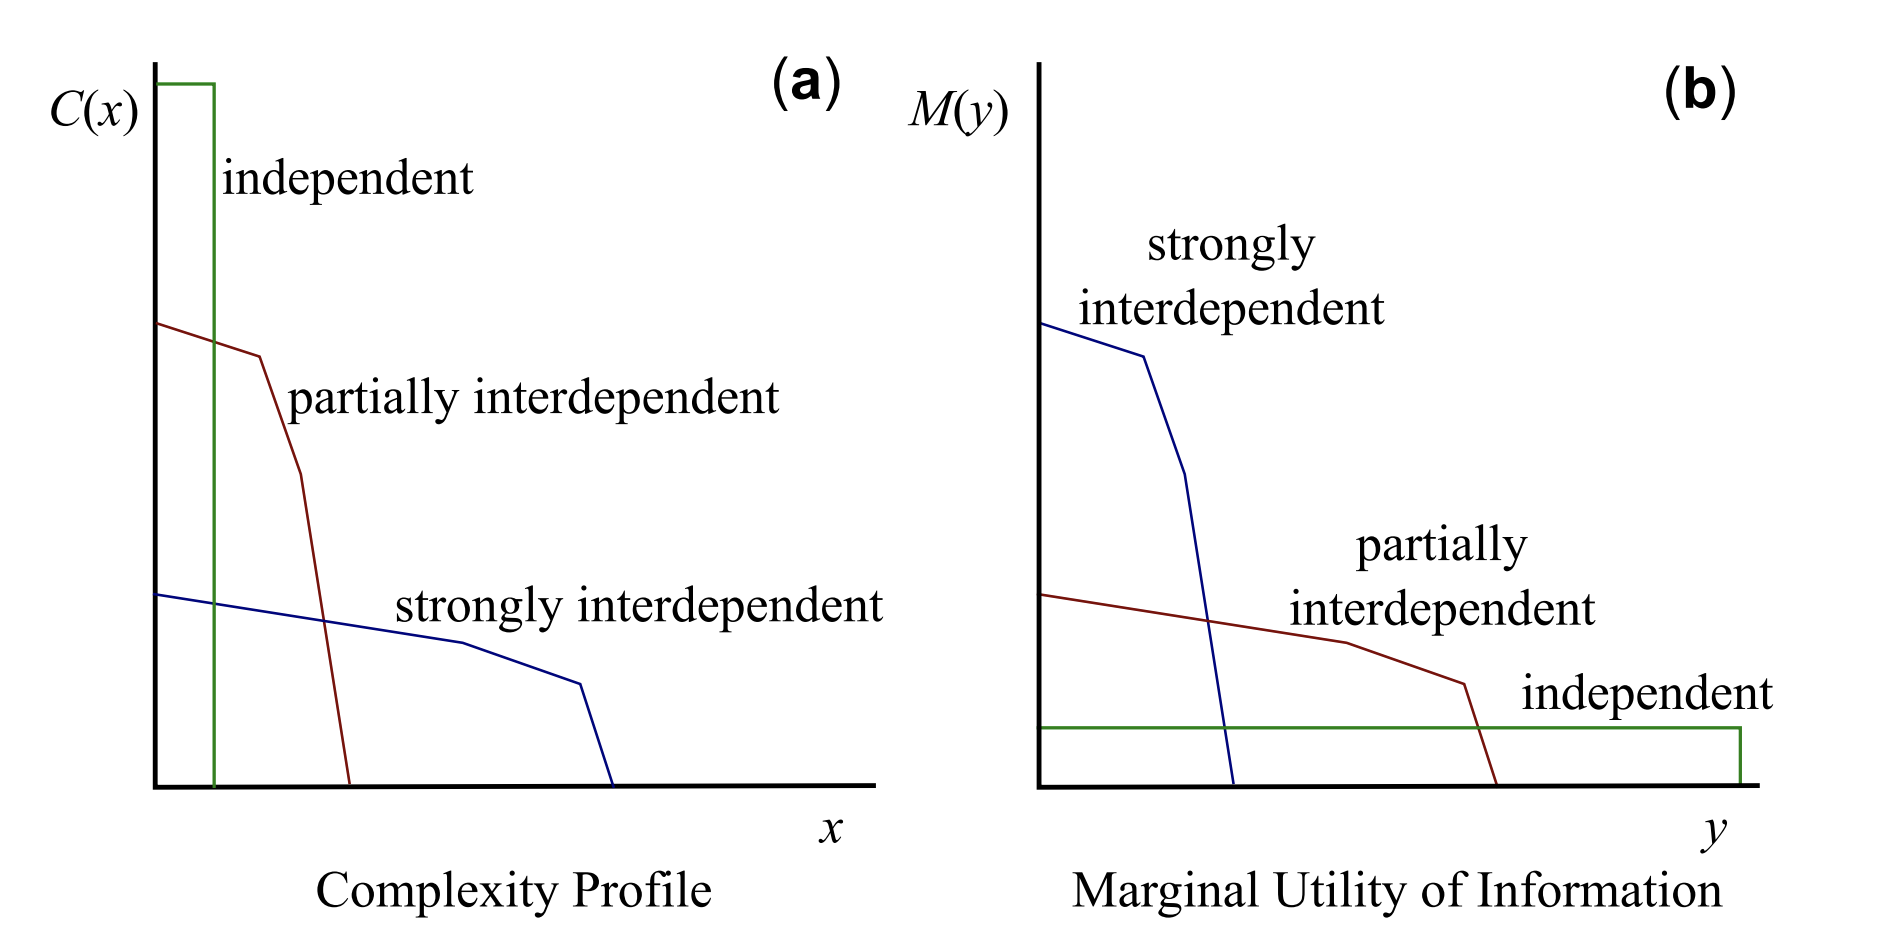
\includegraphics[width=0.8\textwidth]{figures/multiscaleinfo.png}

\cite{allen2017multiscale}

}



%D'autres approches moins formalisées insistent également sur le rôle de la hiérarchie, comme \cite{morin1980methode} qui montre la tension entre dépendance et indépendance d'un organisme à ses constituants, à l'ensemble des niveaux.


\sframe{Complexité Morinienne}{


}






%Il fait alors difficilement sens de proposer que le concept de hiérarchie serait entièrement exogène. En termes d'aide à la décision, et notamment en termes de structures sociales ou politiques, la remise en question complete de la hiérarchie associée aux propositions d'organisations purement horizontales, n'est ni basée sur des faits ni compatible avec les théories de la complexité, en opposition avec les besoins actuels de modèles multi-scalaires pour l'intelligence territoriale soutenable \citep{rozenblat2018conclusion}.

%Ainsi, des approches plus intégratives, larges dans la portée des systèmes considérés, et basées sur les faits, ne peuvent complètement déconstruire le concept de hiérarchie de par son endogénéité à la complexité.


\sframe{Discussion}{

}







\section{Conclusion}


\sframe{Conclusion}{

\justify

\small

$\rightarrow$ 

\bigskip

\footnotesize

\textbf{Références}


%Raimbault, J. (2018). Calibration of a density-based model of urban morphogenesis. PloS one, 13(9):e0203516

\bigskip


%\footnotesize{ - Code, données et résultats disponibles à\\ \texttt{https://github.com/JusteRaimbault/SpatialComplexity}\\
% - Article à \texttt{https://github.com/JusteRaimbault/SpatialComplexity/Docs/}\\\texttt{Rochebrune2019/Versions/Rochebrune2019{\_}Raimbault{\_}v1.pdf}\\
%- Remerciements à \textit{European Grid Infrastructure} et ses \textit{National Grid Initiatives} (\textit{France-Grilles} en particulier) pour le support technique et l'infrastructure.
%}

}








%%%%%%%%%%%%%%%%%%%%%
\begin{frame}[allowframebreaks]
\frametitle{References}
\bibliographystyle{apalike}
\bibliography{biblio}
\end{frame}
%%%%%%%%%%%%%%%%%%%%%%%%%%%%










\end{document}







